\section{24GHz experiments}\label{ghz-experiments}

\subsection{Background}\label{background}

Before going into an account of the the project, let us look at some of
the pros and cons of using this equipment and what is already
known about wireless transmission in the 24 GHz spectrum. We have
already noted that the equipment is affordable. The advertised
throughput of 1.4Gb/s presumably means 700Mb/s in each direction, but
that would provide a satisfactory connection for a hundred or
so residences. Moreover, transmission in this frequency is much
less likely to be affected by tidal reflection (a significant problem
in the Highlands and Islands)

There are some significant drawbacks, though.

\begin{itemize}
\item
  In the UK, the 24.050--24.250GHz band is partitioned into two
  sub-bands, although the 24GHz spectrum is unlicenced the power 
  limits are such that it is unlikely that this equipment would be 
  effective over the distances we have in mind. We obtained a 
  ``non-operational'' licence from Ofcom in order to test the
  equipment  at the advertised power.
\item
  Several of the links used by Tegola and related projects are longer 
  than 13km
\item
  Transmission in higher frequencies is adversely affected by high 
  humidity and high temperatures. Scotland benefits from only one of 
  these.
\item
  The Ubiquiti equipment uses substantially more power than their 5GHz 
  offerings -- about 40W. This would make it unsuitable for solar and 
  wind-powered relays.
\end{itemize}

Our initial plan was to test the equipment on existing Tegola
relays one is a 6.5km link; the second 15.5km. Although the latter is
over the advertised range, even a substantial fraction of the
advertised throughput would be useful.

The following is a roughly chronological account of the project.
The initial installation was done during a period of very high winds
in early January 2014.

\subsection{Initial configuration and testing}
\label{december-2013-initial-configuration-and-testing}

\begin{wrapfigure}{r}{0.3\textwidth}
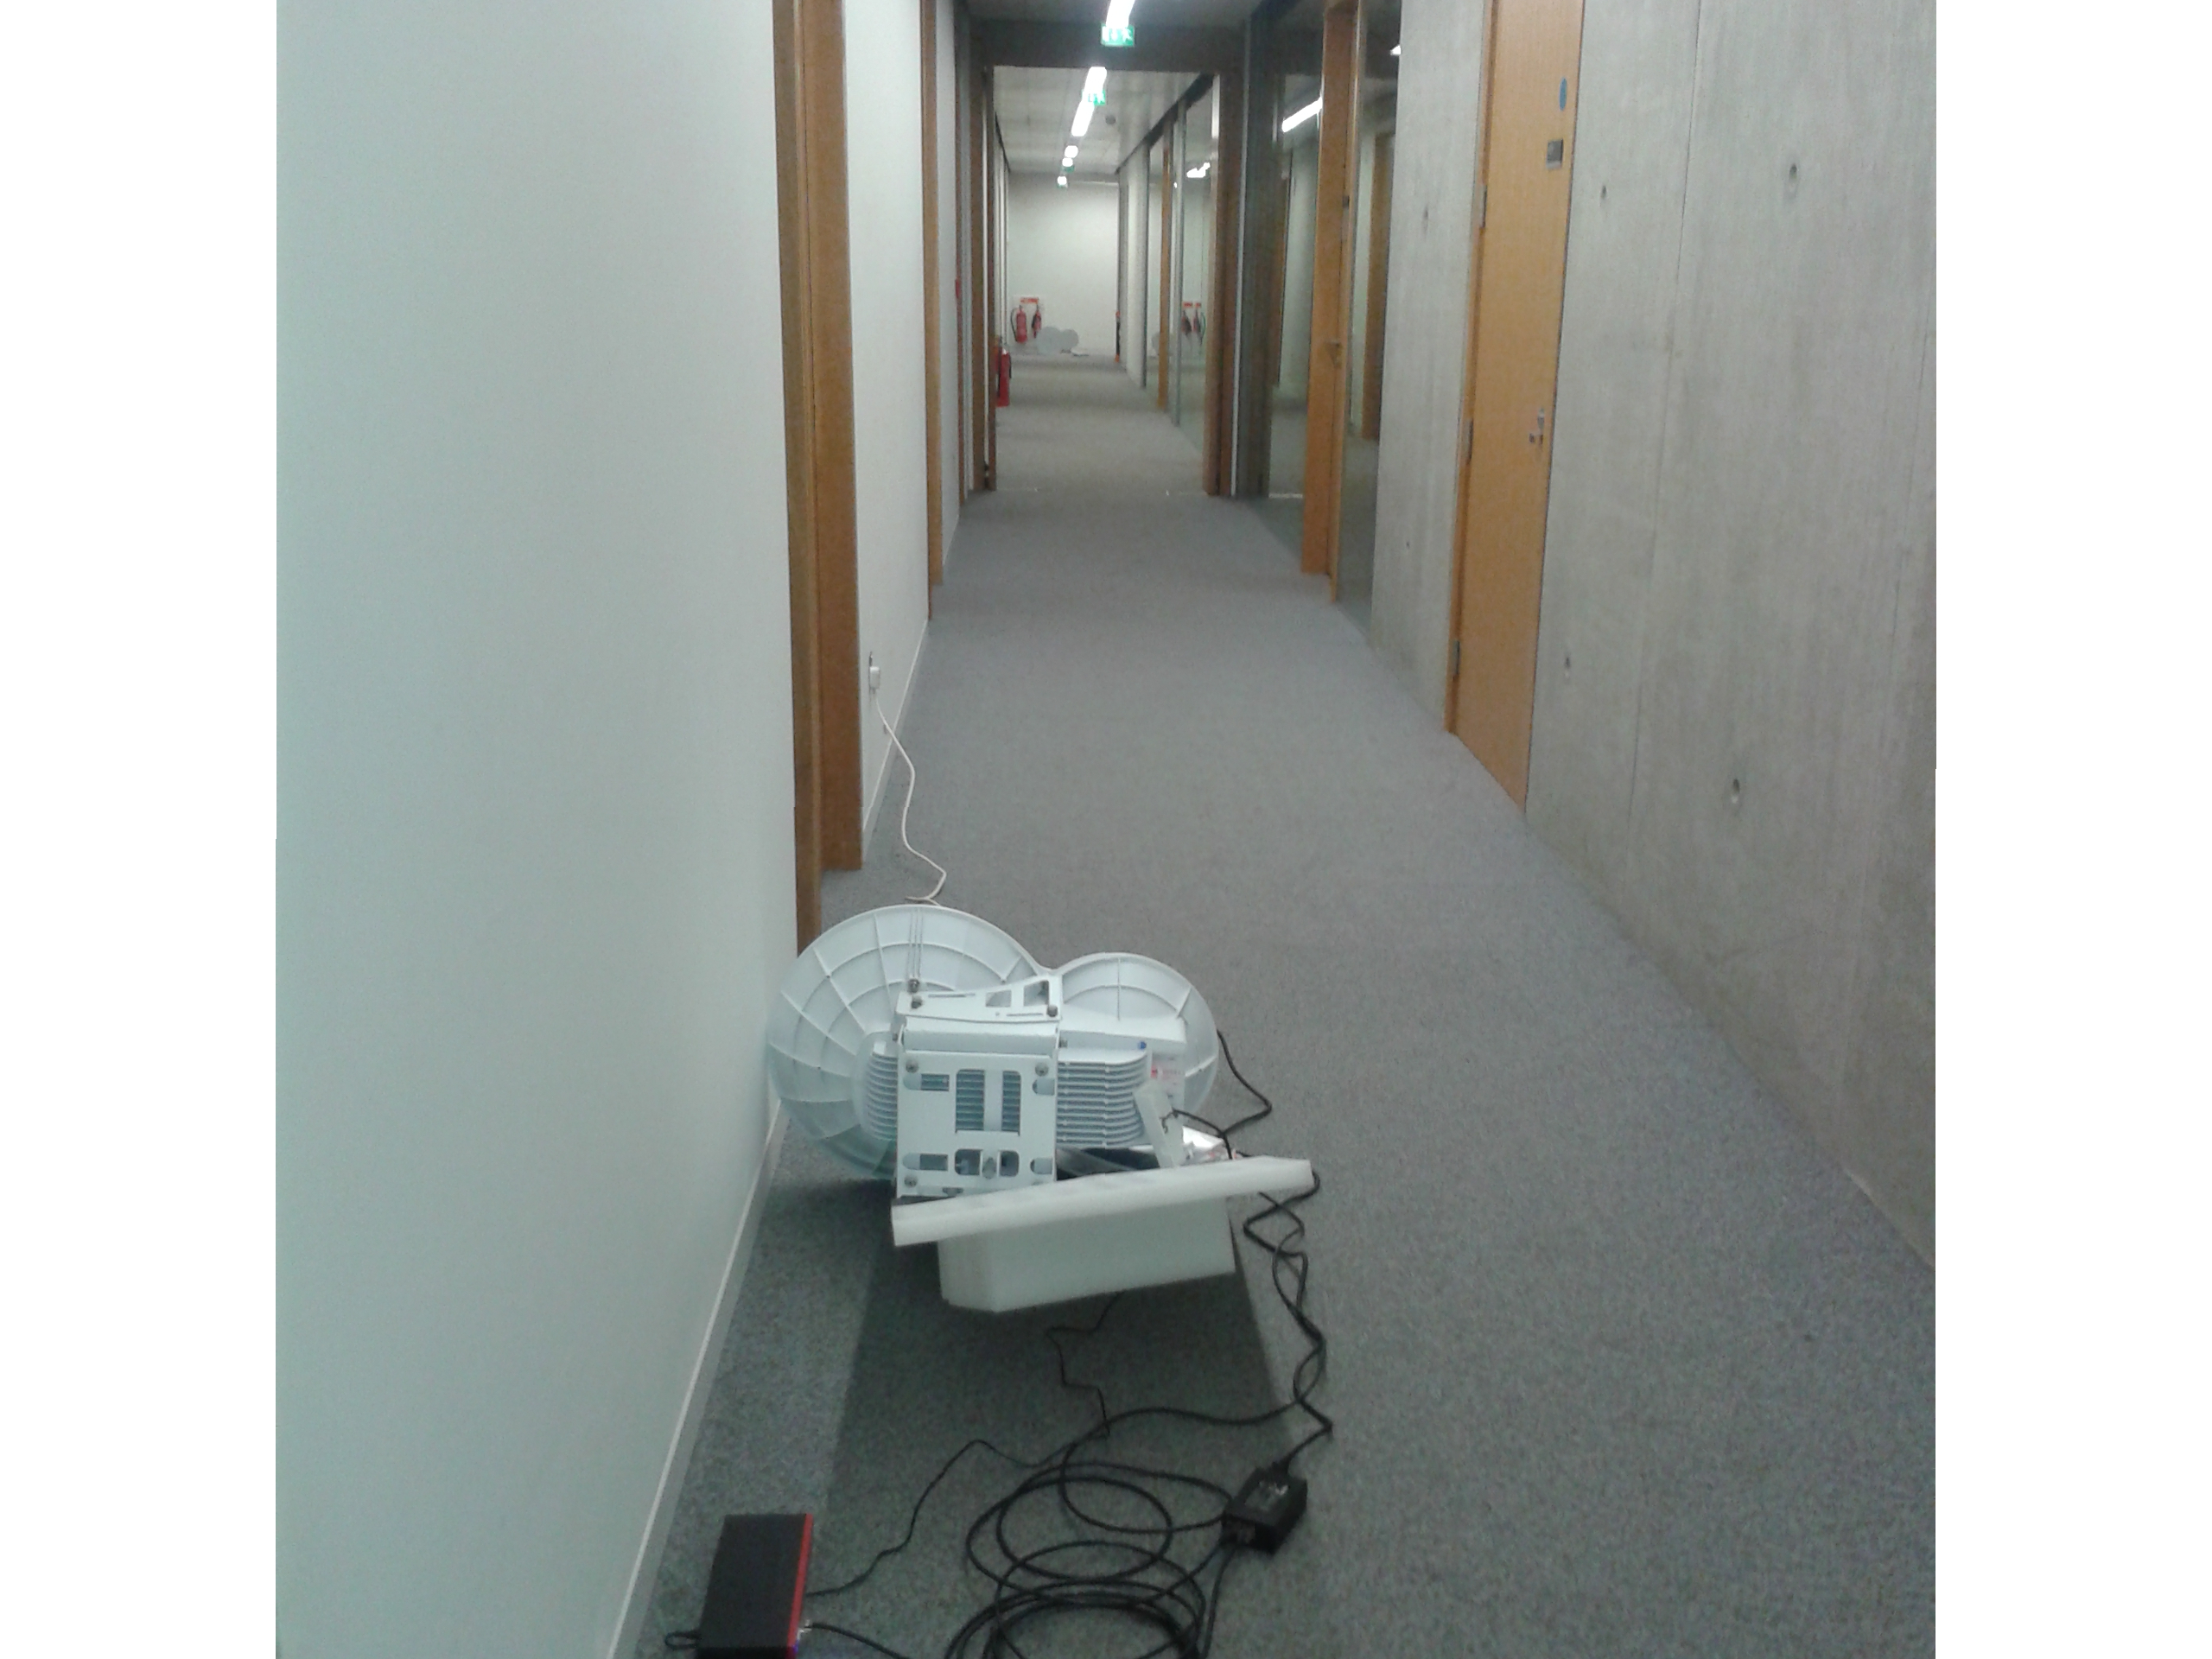
\includegraphics[width=0.3\textwidth]{radio-in-corridor}
\end{wrapfigure}
We ordered and received one pair of radios. Before deploying them
we thought it would be a good idea to check that they were working
and test them in ideal situation -- our office corridor. One thing
we immediately noticed was how critical alignment is. Even over
a distance of 35m, the performance fell of dramatically if the
antennae were slightly out of alignment. It's a very good idea to
configure equipment before deploying it, but to do this we had to turn
off sychronisation which relies on GPS and doesn't work indoors.

\subsection{Strengthening the masts}
\label{december-2013-january-2014-strengthening-the-relays}

Our basic relay construction (see the
\href{http://www.tegola.org.uk/howto/relay-construction.html}{relevant
  howto on the Tegola web site}) uses aluminium pegs to anchor the
diagonal braces to the ground. Both sites were on terrain that
consisted of bedrock covered by peat of varying depth. Although we
have never had a problem with the pegs shifting, peat is a bit
jelly-like, and the structures can wobble through a cm or two. The
alignment of 24GHz is much more critical than for the lower bandwidths
of 2.4 and 5.8GHz, so we replaced the pegs with epoxy bolts into the
bedrock.
\begin{figure}[h]
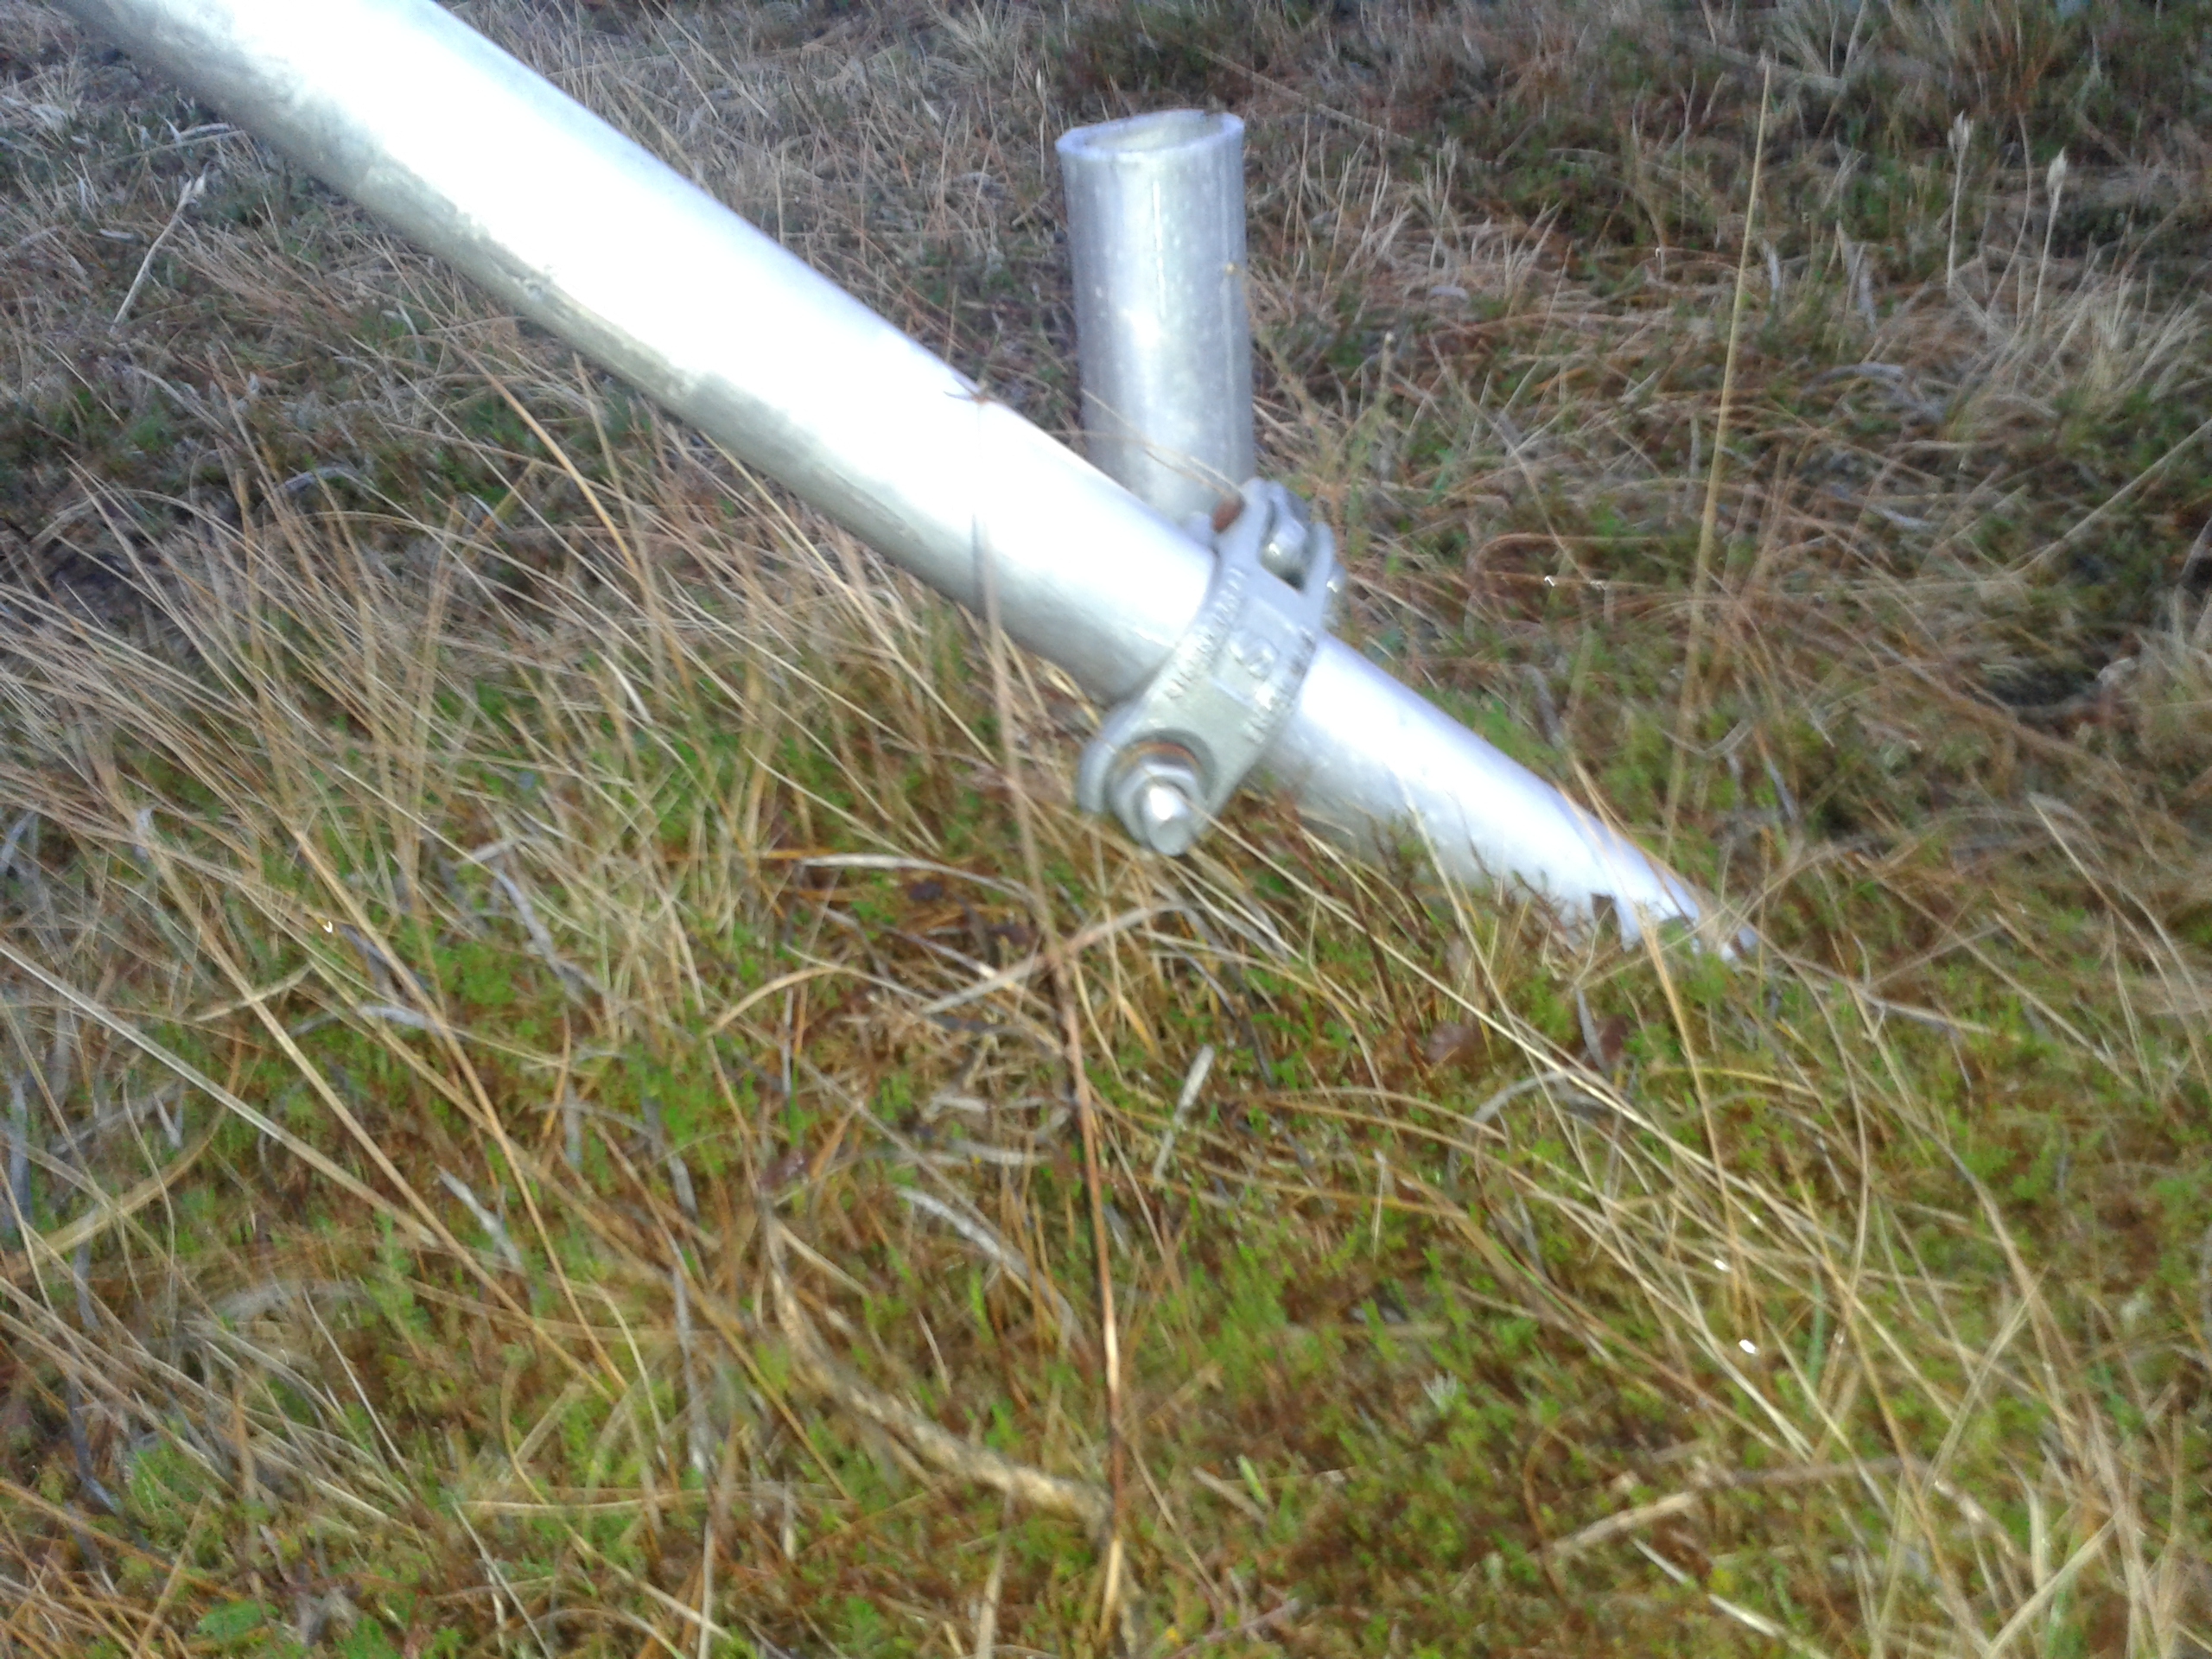
\includegraphics[width=0.4\textwidth]{corran-peg}
\includegraphics[width=0.4\textwidth]{corran-epoxy}
\caption{Pegged anchors (left) and epoxied anchors (right).}
\end{figure}

We also strengthened both relays. For example, at one of our relays we
added an extra horizontal bar.

\begin{figure}[h]
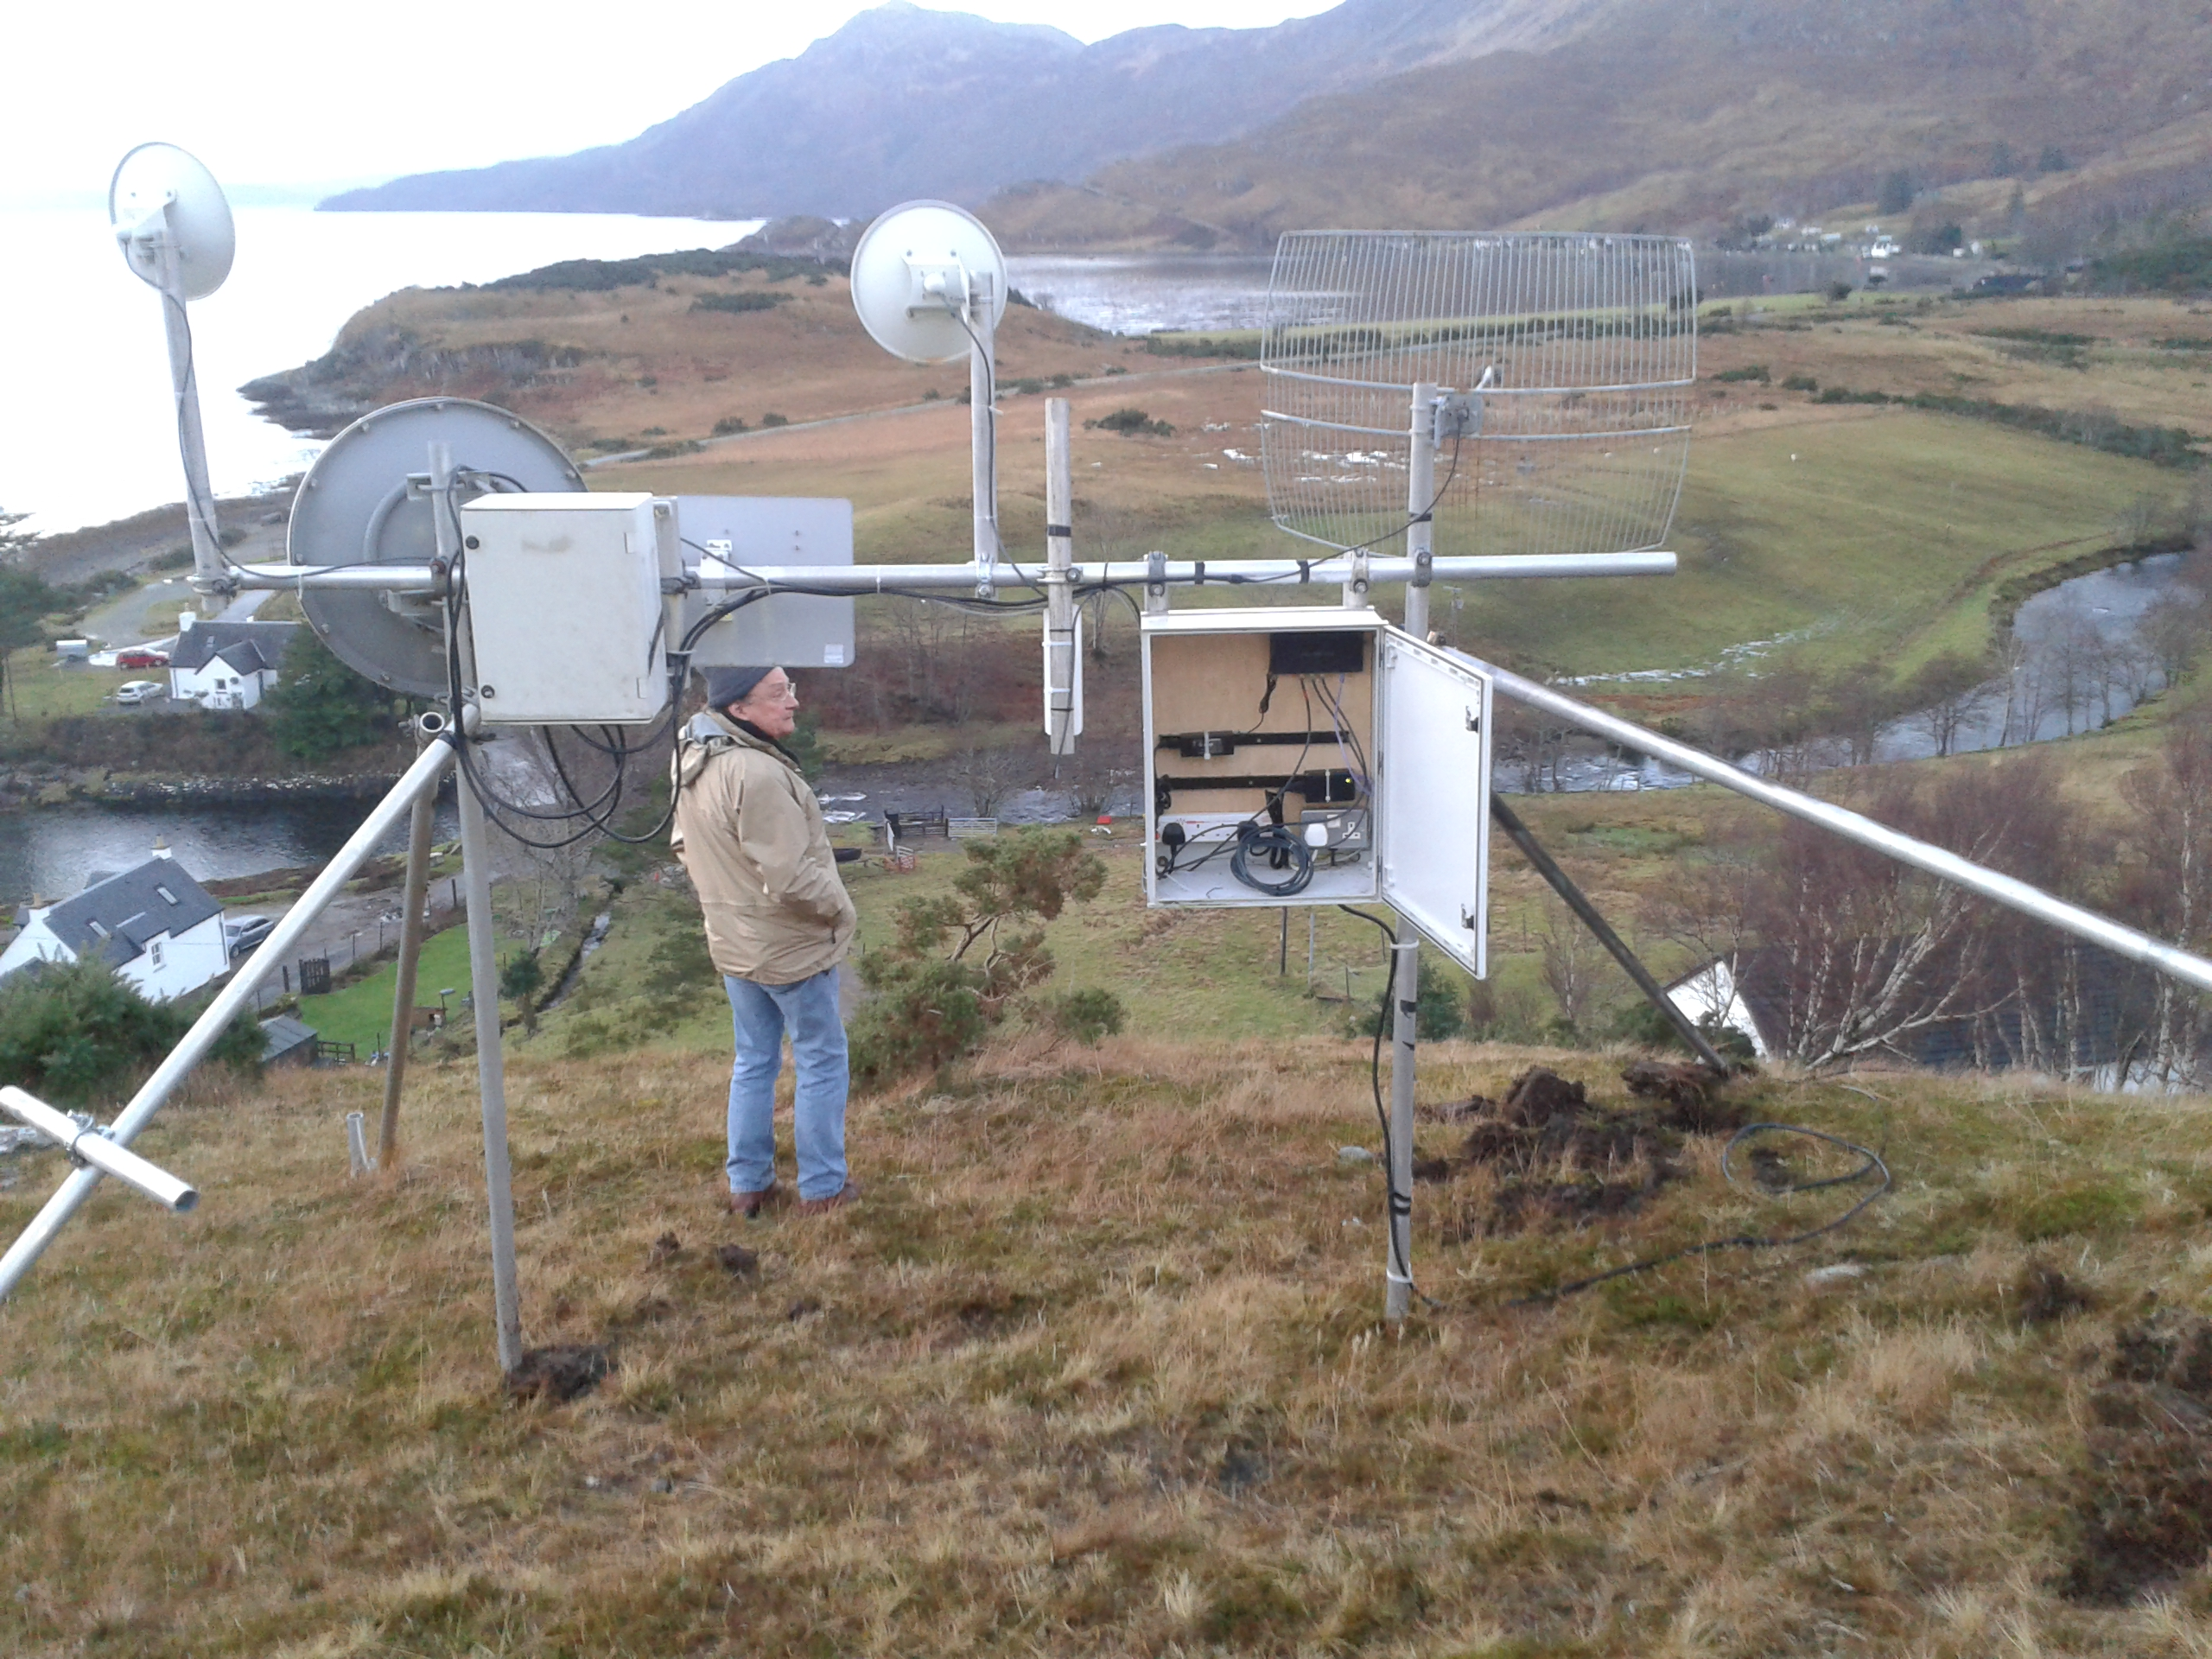
\includegraphics[width=0.4\textwidth]{corran-before-from-behind}
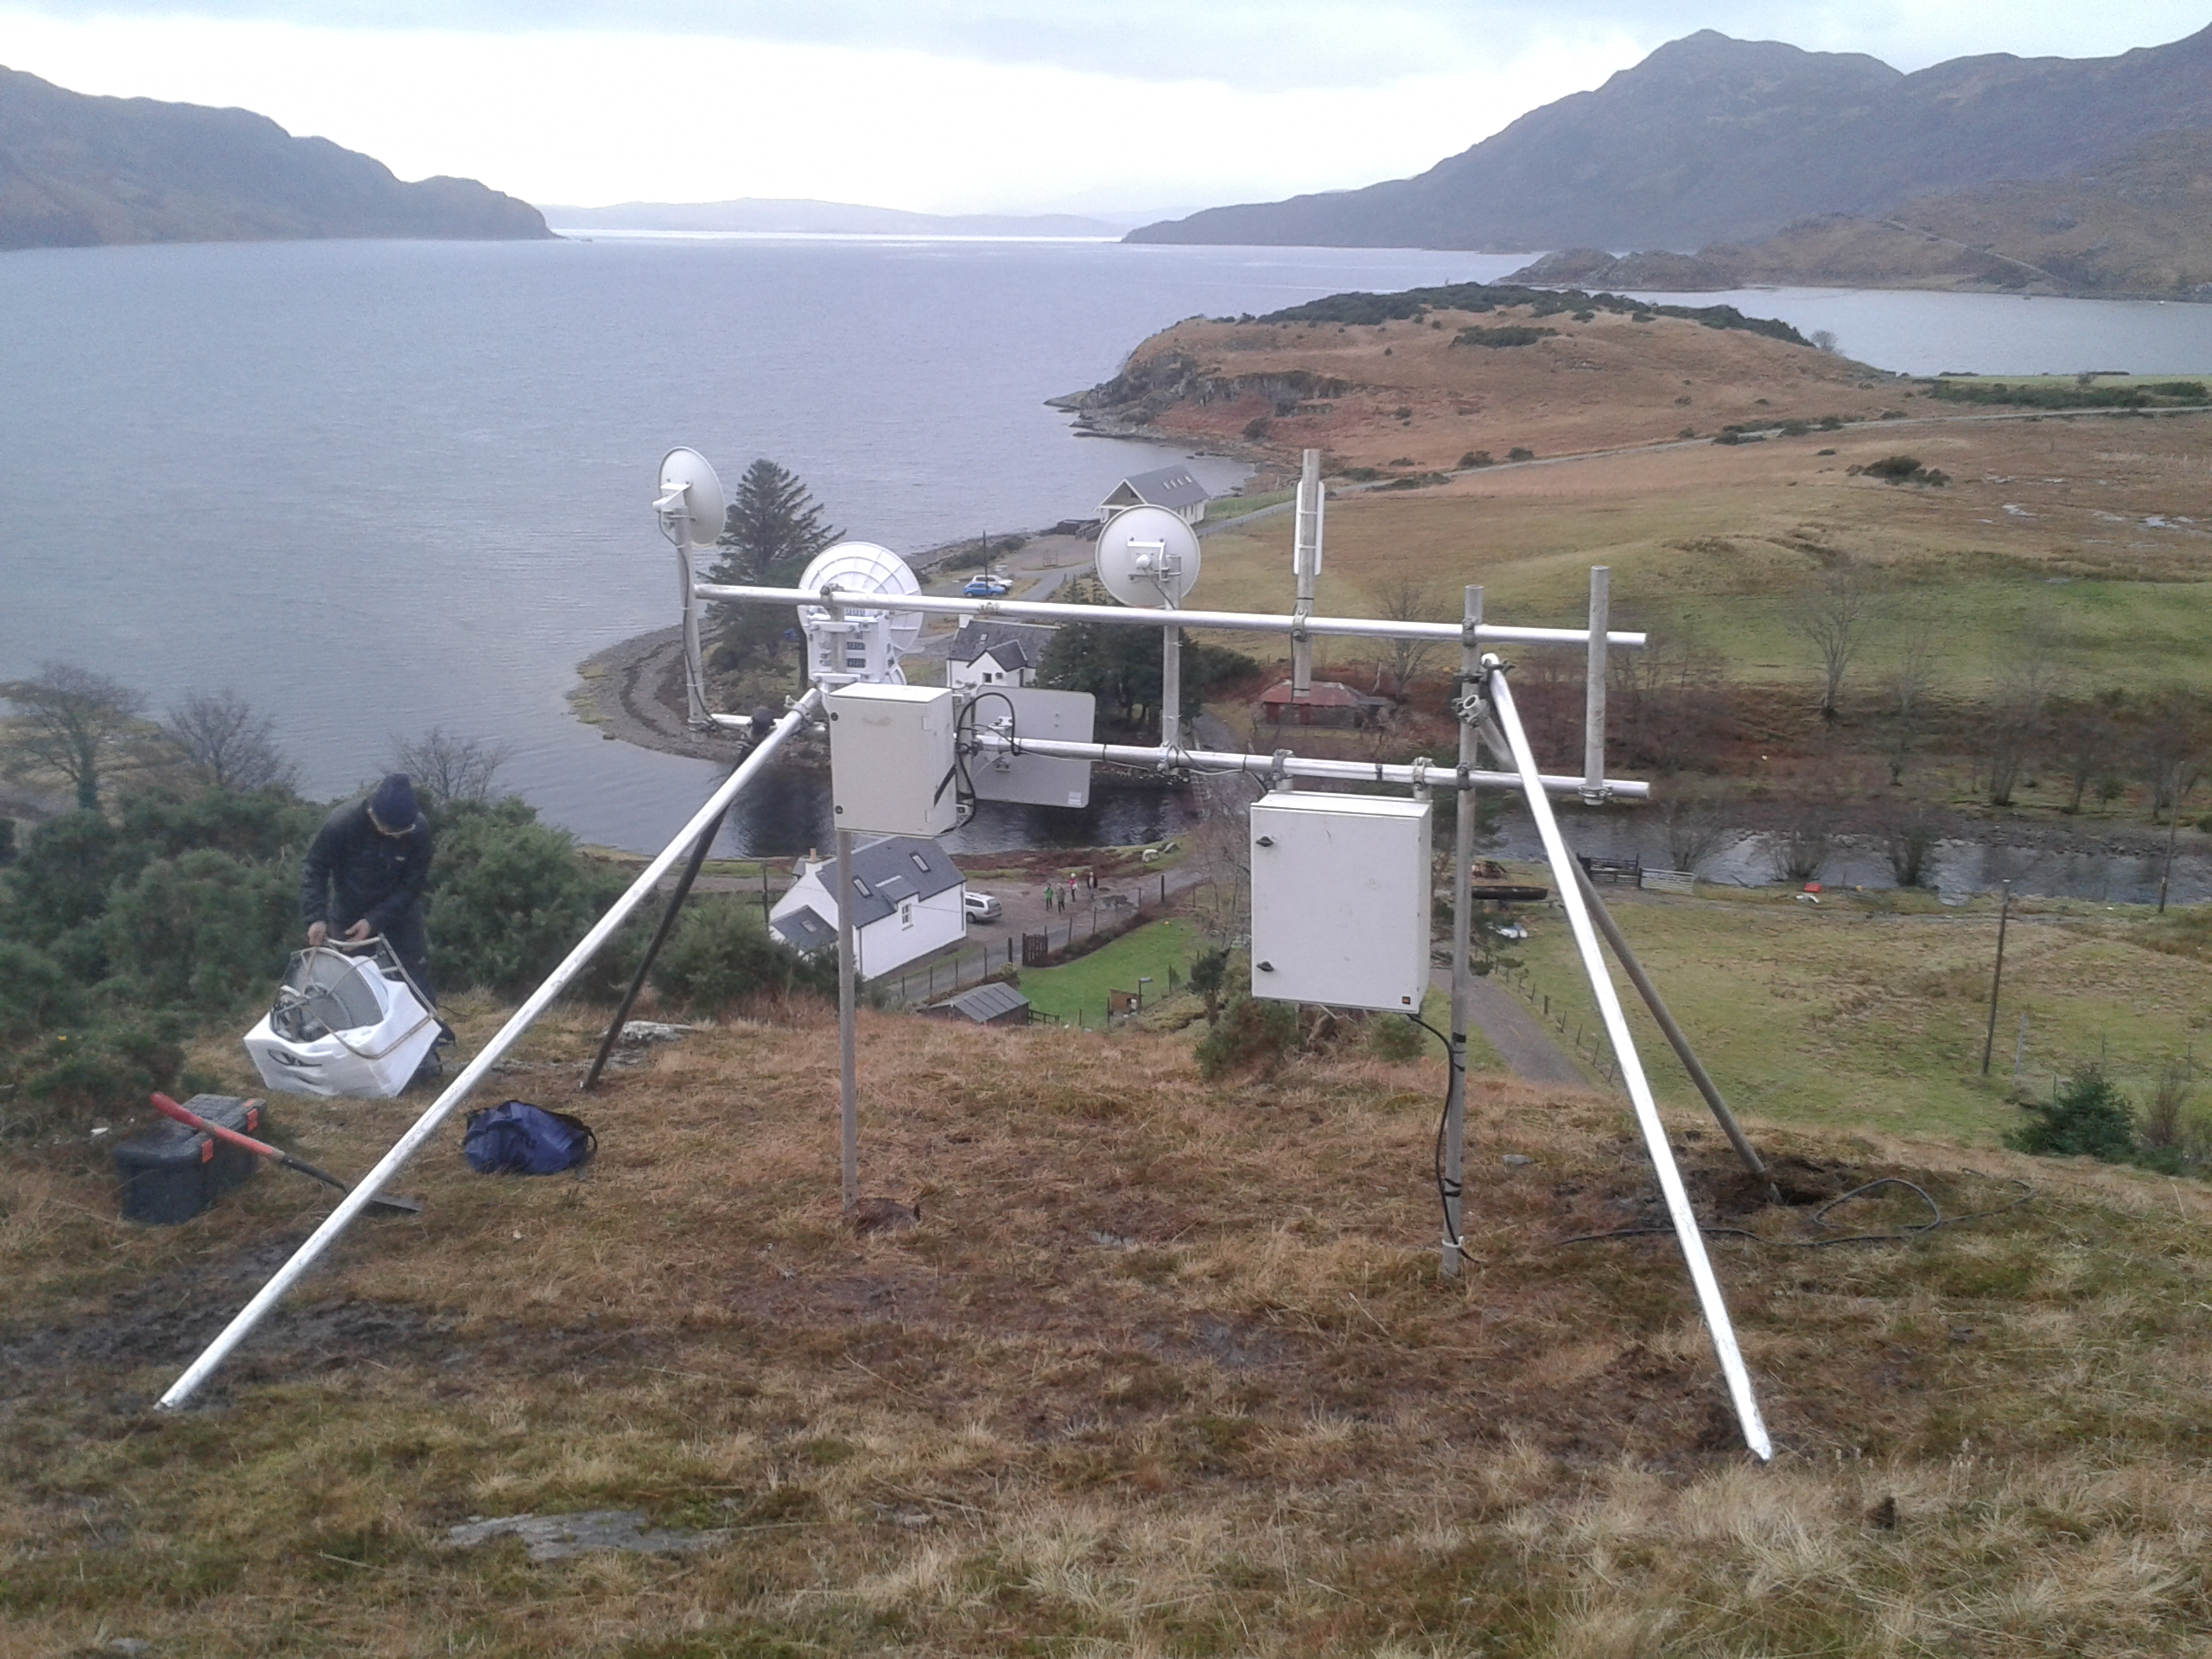
\includegraphics[width=0.4\textwidth]{corran-after-from-behind}
\caption{Corran mast before (left) and after (right)}
\end{figure}

\subsection{Installation and alignment}
\label{january-2014.-installation-and-alignment}

The radios are reasonably light (under 10kg) but awkward to carry up
hills. We used an old backpack frame that 30 years ago had been used
for carrying batteries up to community TV relays. The radios come with
a mounting frame that is first attached to the structure. The radio is
then ``slotted'' into the mounting frame. This arrangement makes it
quite easy to install the whole assembly when working from a ladder.

The antenna can be aligned through elevation and azimuth
adjustment screws. Unfortunately there is a great deal of backlash in
these screws, and they are almost useless if you are working in high
winds. If the clamping bolts are loose, the antenna is blown around
through the considerable travel allowed by the adjustment screws. The
signal strength read-out is at the bottom of the antenna, and if
the alignment is being done from a ladder, you almost certainly
need someone below (with a hard hat) to squint up and call out
the figures.

The installation instructions recommend an alternating process in which
one end of the link is adjusted then the other, and so
on. Unfortunately we were unable to complete this process before
the weather closed in and our workforce departed. However, the
alignment is good enough that we can start taking some measurements.
The initial indications are that the link will work reasonably well
over a distance of 6.5km.

\subsection{Performance}\label{performance}
